% TODO:
% [ ] diagram of sequential AST building process
% 


\section{Program Synthesis}

\begin{itemize}
    \item describe the overall problem. here we start from basic primitives. we are given a few examples of io specifications and the goal is to construct an AST that represents a program, which solves the given task.
    \item What is an AST
    \item What is a DSL 
    \item What is a CFG
    \item What is a PCFG
\end{itemize}

\subsubsection{CFG}

1. Background and Introduction

The field of programming has always been underpinned by the intricacies of formal grammars. Context-Free Grammars (CFGs), a subset of formal grammar, are essential in defining the syntactical structures of many programming languages. However, given the generative nature of CFGs, the potential program space defined by even a modestly complex grammar can be immensely vast. Searching for a specific program within this space, or ensuring that a particular space is sufficiently explored, poses significant computational challenges.

2. Problem Definition

2.1 CFG and Program Space

Let \( G = (N, \Sigma, P, S) \) be a Context-Free Grammar, where:
\begin{itemize}
    \item \( N \) is a finite set of non-terminal symbols.
    \item \( \Sigma \) is a finite set of terminal symbols with \newline \( N \cap \Sigma = \emptyset \)
    \item \( P \) is a finite set of production rules, where each rule is of the form \( N \rightarrow (N \cup \Sigma)^* \)
    \item \( S \) is the start symbol, with \( S \in N \)
\end{itemize}

Given such a CFG, the derived program space \( \Pi(G) \) is the set of all possible strings (or sequences of symbols) derivable from \( S \).

2.2 Problem Statement

Given a Context-Free Grammar \( G \) and a defined objective function \( f \) that maps any program \( p \in \Pi(G) \) to a real value representing its desirability or fitness:

Find \( p^* \) such that:
\[ p^* = \arg\max_{p \in \Pi(G)} f(p) \]

In other words, the problem is to locate a program \( p^* \) within the vast program space \( \Pi(G) \) defined by \( G \) that maximizes (or, alternatively, minimizes) the objective function \( f \).

3. Challenges and Complications

3.1 Size of the Search Space

The generative capacity of CFGs means that even grammars of moderate complexity can define immensely vast program spaces. The sheer size of these spaces poses computational and search challenges.

3.2 Non-Linearity and Discontinuities

The mapping between programs and their fitness as defined by \( f \) might be non-linear with multiple local maxima, making search strategies based on gradient ascent or other linear heuristics suboptimal.

3.3 Generalization vs Specification

While CFGs provide a generalized representation of possible programs, the objective function might lead to highly specialized solutions. Balancing between the two is non-trivial.

3.4 Syntactic vs Semantic Validity

A CFG ensures syntactic validity but does not guarantee semantic correctness. Ensuring that a program derived from a CFG is semantically meaningful or error-free in a given context is an additional layer of complexity.

\begin{itemize}
    \item How are programs represented (ASTs, GNNs, other ideas from different papers)
    \item Tree-Transformers
    \item 
\end{itemize}

% Here we talk about program synthesis and previous approaches

Rewrite the following:
Program synthesis is a notoriously challenging problem. Its inherent challenge lies in two main components of the problem: intractability of the program space and diversity of user intent.

%Program Space In its most general formulation (for a Turing-complete programming language and an arbitrary constraint) program synthesis is undecidable, thus almost all successful synthesis approaches perform some kind of search over the program space. This search itself is a hard combinatorial problem. The number of programs in any non-trivial programming language quickly grows exponentially with program size, and this vast number of possible candidates for a long time has rendered the task intractable. Early approaches to program synthesis focused on deductive and transformational methods [85, 86]. Such methods are based on a exponentially growing tree of theorem-proving deductive inferences or correctness-preserving code rewrite rules, respectively. Both approaches guarantee that the produced program satisfies the provided constraint by construction but the non-deterministic nature of a theorem-proving or code-rewriting loop cannot guarantee efficiency or even termination of the synthesis process. Modern successful applications of similar techniques employ clever domain-specific heuristics for cutting down the derivation tree (see, for example, [63, 104]). The last two decades brought a resurgence of program synthesis research with a number of technological and algorithmic breakthroughs. First, Moore's law and advances in constraint solving allowed exploring larger program spaces in reasonable time. This led to many successful constraint-based synthesis applications tracing their roots back to Sketch and the invention of counterexample-guided inductive synthesis [132]. Second, novel approaches to program space enumeration such as stochastic techniques [105, 123] and deductive top-down search [43, 113] enabled synthesis applications in new domains that were difficult to formalize through theorems and rewrite rules. However, even though modern-day synthesis techniques produce sizable real-life code snippets, they are still rarely applicable to industrialsize projects. For instance, at the time of this writing, the state-of-the-art superoptimization technique (i.e., synthesizer of shorter implementations of a given function; see §2.6) by Phothilimthana et al. [109] is able to explore a program space of size 1079. In contrast, discovering an expert implementation of the MD5 hash function requires exploring a space of 10^5943 programs!1 New algorithmic advances and clever exploitation of domain-specific knowledge to facilitate large program space exploration is an active research area in program synthesis.


Statistical Various kinds of statistical techniques have been proposed including machine learning of probabilistic grammars, genetic programming, MCMC sampling, and probabilistic inference. Machine learning techniques can be used to augment other search methodologies based on enumerative search or deduction by providing likelihood of various choices at any choice point. One such choice point is selection of a production for a non-terminal in a grammar that specifies the underlying program space. The likelihood probabilities can be function of certain cues found in the input-ouput examples provided by the user or the additionally available inputs [89]. These functions are learned in an offline phase from training data. Genetic programming is a program synthesis method inspired by biological evolution [72]. It involves maintaining a population of individual programs, and using that to produce program variants by leveraging computational analogs of biological mutation and crossover. Mutation introduces random changes, while crossover facilitates sharing of useful pieces of code between programs being evolved. Each variant's suitability is evaluated using a user-defined fitness function, and successful variants are selected for continued evolution. The success of a genetic programming based system crucially depends on the fitness function. Genetic programming has been used to discover mutual exclusion algorithms [68] and to fix bugs in imperative programs [146] MCMC sampling has been used to search for a desired program starting from a given candidate. The success crucially depends on defining a smooth cost metric for Boolean constraints. STOKE [124], a superoptimization tool, uses Hamming distance to measure closeness of generated bit-values to the target on a representative test input set, and rewards generation of (almost) correct values in incorrect locations. Probabilistic inference has been used to evolve a given program by making local changes, one at a time. This relies on modeling a program as a graph of instructions and states, connected by constraint nodes. Each constraint node establishes the semantics of some instruction by relating the instruction with the state immediately before the instruction and the state immediately after the instruction [45]. Belief propagation has been used to synthesize imperative program fragments that execute polynomial computations and list manipulations [62].

\cite{gulwani_program_2017}



% Several techniques have emerged as pivotal in the domain of program synthesis:

% Deductive Synthesis: Rooted in formal logic, this method transforms specifications into programs. The use of logic mirrors certain cognitive tasks, especially those demanding strict reasoning.

% Stochastic Search: By randomly exploring the space of possible programs, these methods mirror heuristic-based cognitive processes. Genetic algorithms, for instance, mimic evolutionary processes to evolve optimal or near-optimal solutions.

% Neural Program Synthesis: Neural networks, especially recurrent ones, have shown promise in generating programmatic structures. The parallels between neural networks and neural structures in the brain offer tantalizing possibilities for cognitive science.

% Example-Based Synthesis: Drawing inspiration from how humans often learn—from examples—these methods generate programs by generalizing from provided instances. This mirrors pedagogical processes and experiential learning.





\subsection{EM}
In the exact EM, the distribution is stored as a matrix of logits, in the variational EM it is represented as parameters of a simpler distribution, and in the amortized variational EM, it is represented as the weights of a neural network.

\subsection{DreamCoder}
DreamCoder (DC) is a model that synthesises programs from initial primitives in a domain specific language (DSL) and a set of tasks \cite{ellis_dreamcoder_2021}. The model utilises a modified version of a wake-sleep algorithm \cite{hinton1995wake} to learn a generative model and a recognition network in tandem. The generative model learns a probability distribution over programs while the recognition network learns to map from tasks to programs and serves as neurally guided search over the program space.
DreamCoder builds its library of programs from primitives in its DSL, and creates higher-order functions.
Sub-routines that are commonly used, are chunked and abstracted into concepts which become more accessible. This narrows the search tree immensely and enables scalability.

- hypothesis space
- learning its own dsl

Tasks can be generative (e.g. creating an image) or conditional, (input-output relation, e.g. sorting a list).
% Figure \ref{LaTeX/img/conc_library.png}(A) shows examples of tasks across different domains. 
% Figure \ref{fig:../img/conc_library}(B) shows an example, in which the task to learn is to sort a list. On the left we see the initial primitives. The shaded region shows the learned library of concepts. On the right we see the final solution, which uses \texttt{concept15} , which itself uses previously abstracted concepts. Note the difference in the length of the program using abstracted concepts vs. only initial primitives, shown beneath.

% \begin{figure*}
% 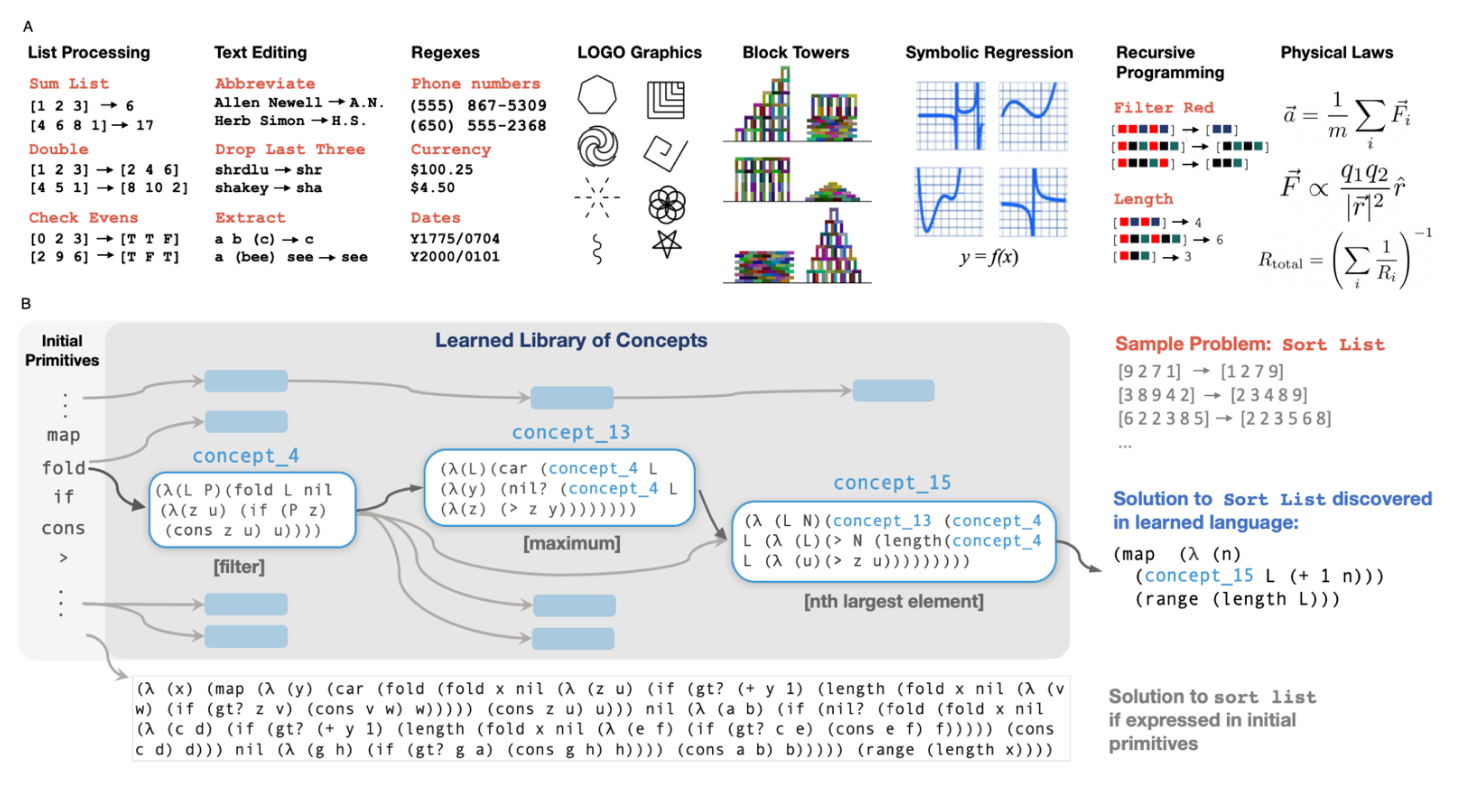
\includegraphics[width=\textwidth]{img/conc_library.png}
% \label{fig:conc_library}
% \caption{(A) 8 different domains of tasks. (B) Representation of the learned library of concepts. On the left we see the initial primitives from which the concepts in the middle region are composed. On the right we see a task as input-output relations and the found solution. On the bottom is the same solution expressed only with initial primitives. Image taken with permission from the original paper \cite{ellis_dreamcoder_2021}.}
% \end{figure*}

The model operates in three distinct phases. 

\paragraph{Wake} In the wake phase, the objective is to find the best program $\rho$  for each task $x \in X$ DreamCoder is presented with. Each task consist of one or a few (up to $\sim10$) examples. The system synthesises the programs using a neural network as the recognition model $Q$ to search through its library $D$.

\paragraph{Sleep: Abstraction} A key component of the success of DreamCoder is the refactoring of programs. In this phase, DreamCoder consolidates new abstractions from the programs it has found during the wake phase. Experiences are replayed, and commonalities between programs are found so that they can be abstracted into new concepts to use in the future. The objective is to find programs of minimum description length (MDL). 

\paragraph{Sleep: Dreaming} The objective during the dreaming phase is to train the recognition model $Q$ to perform MAP inference by both fantasies, and replays. When fantasising, programs are drawn from the learned library as a generative model. The model is then trained on the produced tasks. This ensures a large and varied data-set to learn from and encourages out-of-distribution generalisation. Replays, simply training on previously seen task-program pairs, ensures that the model improves its predictions on the actual tasks it needs to learn, by using its programs.

A Bayesian View
- What exactly happens?
- The generative model is a CFG, parameterized my a 
Include the parameterization of the generative model as a bigram transition matrix (three dimensional. Parent, arg index, depth?)





% “We use an EM algorithm to estimate the continuous parameters of the generative model, i.e. θ. Suppressing dependencies on D, the EM updates are θ = arg max θ log P (θ) + ∑ x Eqx [log P [ρ|θ]] (3) qx(ρ) ∝ P[x|ρ]P[ρ|θ]1 [ρ ∈ Bx] (4) In the M step of EM we will update θ by instead maximizing a lower bound on log P[ρ|θ], making our approach an instance of Generalized EM.” (from building hierarchical world models , one of the DreamCoder papers)



\begin{itemize}
    \item Frontier of primitives and abstracted concepts essentially form a markov blanket. Is that true? 
\end{itemize}

\section{Transformer}

At the heart of the transformer is the self-attention mechanism, which enables the model to weigh the significance of different tokens in a sentence relative to a given token.

$$ \text{Attention}(Q, K, V) = \text{softmax}(\frac{QK^T}{\sqrt{d_k}})V $$
where
\begin{itemize}
    \item $Q$: Query matrix
    \item $K$: Key matrix 
    \item $V$: Value matrix
    \item $d_k$: Dimensions of keys
\end{itemize}

The self-attention mechanism allows the model to focus on different tokens with varying intensities, enabling it to capture long-range dependencies in the data.

Since the transformer lacks inherent notions of sequence order (unlike e.g. RNNs), positional encodings are added to the embeddings at the bottoms of the encoder and decoder stacks. This ensures that the model can attend to the position of words in the sequence. These encodings are added to the embeddings and have the same dimension, enabling the summed values to be processed in the self-attention layers.

Embeddings convert tokens into dense vectors of fixed size, capturing semantic meanings and relationships. This enables the model to understand relationships between different tokens.

\begin{itemize}
    \item Why is attention all you need?
    \item Why is the transformer architecture so relevant in the past few years?
    \item Why does it take away the need for archictecture search
    \item Multi-Head Attention: Instead of a single set of attention weights, the model uses multiple sets, enabling it to focus on different parts of the input for different tasks simultaneously.
    \item Feed-forward Networks: Each layer of the transformer contains a feed-forward neural network, which is applied independently to each position.
    \item Normalization and Residual Connections: These components help in stabilizing the activations and enabling deeper stacking of layers.
    \item Stephen Wolfram explains in his book about ChatGPT and the accompanying blog article how a thought can be seen as a trajectory through semantic space. 
\end{itemize}






%%%%%%%%% METHODS


Recent advancements in program synthesis have seen the rise of novel techniques aimed at generating code that not only satisfies a given specification but also matches human-written code patterns. One of the most notable methods in this sphere is DreamCoder. This model, along with several other state-of-the-art (SOTA) methodologies, has shown exceptional proficiency in understanding and generating complex code structures based on given specifications.

However, a critical examination of such methods, including DreamCoder, reveals a foundational limitation: their heavy reliance on syntactical constraints. While these constraints are undoubtedly vital for ensuring the correctness of generated programs, they do not necessarily guarantee a deep understanding or utilization of semantic relationships within the code. This is akin to learning the grammar of a language but missing out on the nuances and contexts that give meaning to words and phrases.

One could argue that the attention mechanism, as seen in transformers, provides a potential solution to this limitation. The attention mechanism inherently captures dependencies between various parts of an input, no matter how distant they might be. In the context of program synthesis, such a mechanism could be instrumental in deriving and maintaining meaningful semantic relationships between different code segments. The beauty of attention is that it provides a dynamic way to weigh different parts of the input based on context, potentially allowing a transformer-based model to capture intricate semantic details of a program.

Nevertheless, a transformer's capabilities come with its own set of challenges. While the attention mechanism offers a promising avenue for capturing semantic nuances, transformers, especially when trained from scratch, require colossal amounts of data to achieve satisfactory performance. The fundamental architecture of transformers necessitates this data-driven learning, often demanding diverse and extensive training datasets that might not always be available or feasible, especially in niche areas of program synthesis. Moreover, when the goal is to create a model of human cognitive abilities, it is obvious that humans do not have access to vast amounts of data, instead, we are able to infer causal relationships, from only a limited number of examples. E.g. consider the problem \texttt{[1,2,3] $\rightarrow$ [3,2,1]}. An astute reader might promptly conclude that the list has been reversed \rephrase[inline]{maybe that's a bit smug}. 
Dougs analogies 

This is where GFlowNets (GFNs) carve their niche. Contrary to the data-hungry nature of transformers, GFNs do not necessitate gargantuan datasets for efficient training. Instead, they leverage a more intuitive approach: defining a reward distribution that's directly proportional to the objects (or programs) we intend to generate. This not only streamlines the learning process but also ensures that the synthesized programs are aligned with our desired outcomes.

In the realm of program synthesis, our objectives are clearly defined. We aim to construct objects, or more specifically, pieces of code that precisely meet the given specification. This isn't just about producing syntactically correct code; it's about generating semantically rich and efficient programs that can effectively solve the specified problem without superfluous or redundant components.







\begin{itemize}
    \item What is the problem? why can't we marginalise over the CFG? or can we? 
    \item How does GFN or DC deal with it? 
\end{itemize}



In DreamCoder, they do something similar. They have a generative model in the form of a PCFG, and a recognition model which takes a task as input and outputs a bigram transition tensor, which serves as a policy over actions. Here $Q$ is a conditional distribution, a mapping between IOs and programs. This is essentially an encoding of programs as tasks, which can also be seen in their visualization of task embeddings.
The PCFG is completely syntactical.
So they train the model to predict better weights and then search in the pcfg enumeratively. 

for each task they have a beam, which they marginalize over. 

What is the prior, likelihood, etc. how is it operationalised

An EM algorithm is used to estimate the parameters of the generative model. 

Explain why they chose a bigram over transformer (efficiency in searching. however one could use transformer without search, but usually some kind of search is necessary. ) related to sample quality over search

Explain why they look for MAP over posterior (symmetry breaking)

\begin{itemize}
    \item argument for attention and why it might be necessary to capture semantics.
    \item transformers learn nested relationships (see chapter wolfram) (relationships of increasing complexity)
    \item 
\end{itemize}

In FlowCoder, I do a couple things differently:

\begin{itemize}
    \item I embed all the rules (check this with neuralPCFG and maybe embed the cfg so that you have a better generative model)
    \item I am searching for the posterior (aligning with active inference), because i want diverse solutions, i.e. i want to learn the solution space for each task, multiple modes, not just the max mode. (how does this compare to MDL)
    \item 
\end{itemize}

\begin{itemize}
    \item does the model align with FEP
    \item If the CFG is generative, is that not a causal model? can there be a generative causal model? be clear about those terms. 
\end{itemize}

%%%%%%%%%%%%%%%%%%%%%%%%%%%%%%%%%%%%
%%%%%%%%%%%%%%%%%%%%%%%%%%%%%%%%%%%%
%%%%%%%%%%%%%%%%%%%%%%%%%%%%%%%%%%%%
%%%%% Algorithmic Description %%%%%%
%%%%%%%%%%%%%%%%%%%%%%%%%%%%%%%%%%%%
%%%%%%%%%%%%%%%%%%%%%%%%%%%%%%%%%%%%
%%%%%%%%%%%%%%%%%%%%%%%%%%%%%%%%%%%%

\section{GFlowNet}
The problem can be formalized as finding a latent hierarchical structure from a limited set of specifications.

We can specify our GFlowNet in the realm of program synthesis as building a directed acyclic graph over abstract syntax trees.
We formalise it. 
The gfn is conditioned on the task, and so we have a conditional reward distribution $R(z|x)$, as well as a conditional forward policy $P_F(s|x)$ and partition function $Z(x)$.

I am building on the DeepSynth framework where the goal is to find programs in a domain specific language. 
The task is list editing, i.e. i get some inputs and outputs relationship and the network has to find a program that solves it. 
we want diversity, so perhaps even multiple programs that solve it.

\section{Theory}

The trained GFlowNet gives us a the stochastic policy $\pi(a|s)$, where $a$ is an action from the action space $A$ and $s$ is a state from the state space $S$.

\begin{itemize}
    \item Relation to MDPs, POMDPs
    \item Relation to Reinforcement learning
    \item Relation to MCMC sampling
    \item Relation to Variational inference. 
\end{itemize}

Since their initial publication [SOURCE], many extended and modified variants have been published. See e.g. [SOURCE, awesome GFlowNets for an overview.]

\section{Methods}

\begin{itemize}
    \item Reasons for using a GFlowNet
    \item Transformer allows for semantic relationships (although we still don't use control or data flow, but we could in principle)
    \item We want to approximate a multimodal distribution, unlike DreamCoder in which the MAP estimate refrains from finding semantically equal but syntactically different solutions.
\end{itemize}





























\section{DeepSynth}




In their 2021 paper, Fijalkow et al. proposed a framework called "distribution-based search", in which they tackle the difficult problem of searching through a DSL to find programs matching a specification in a vast hypothesis space. 

The authors introduce DeepSynth \footnote{\url{https://github.com/nathanael-fijalkow/DeepSynth}}, a general-purpose program synthesizer which constructs programs from input-output examples \cite{fijalkow_scaling_2021}. They make use of a 2-step pipeline in which a neural network learns to predict weights for a context free grammar (CFG), making it a probabilistic CFG (PCFG) and then a search algorithm seeks programs matching the query.

However, rather than trying to improve models for program synthesis, they focus on how to best utilize this neural predictor in order for the system to be useful and scale beyond trivial programs.

\rephrase[inline]{At a high-level the approaches we develop in this work follow a 2-stage pipeline: in the first stage a learned model predicts probabilistic weights, and in the second stage a symbolic search algorithm uses those weights to explore the space of source code. 
Our contributions target the second stage of this pipeline, and we focus on theoretical analysis of sampling-based search algorithms, new search algorithms based on neurally-informed enumeration, and empirical evaluations showing that recent neural program synthesizers can compose well with our methods.}


\begin{itemize}
    \item Loss optimality
    \item Learning the weights of a CFG making it a PCFG, then finding programs using this PCFG. 
    \item There is a trade-off between finding many programs rapidly, or fewer programs that are more likely to solve the problem.
    \item enumeration vs sampling
    \item They show that all sampling algorithms are either loss optimal or have infinite loss?
\end{itemize}

In DeepSynth, we are given a list of primitives, the initial DSL, with a number of syntactic constraints which compile into a context free grammar. they then train a prediction model to predict the weights of the cfg making it a pcfg. lastly they search through the pcfg to find programs meeting the given specification.

\rephrase[inline]{the DSL is given by a set of primitives together with their (possibly polymorphic) types and semantics.
We describe the machine learning pipeline for program synthesis, illustrated in Figure 1 on a toy DSL describing integer list manipulating programs.
The compilation phase constructs a context-free grammar (CFG) from the DSL together with a set of syntactic constraints. The CFG may incorporate important information about the program being generated, such as the n last primitives (encompassing n-gram models) or semantic information (e.g. non- zero integer, sorted list).
A prediction model (typically a neural network) takes as inputs a set of I/O and outputs a probabilistic labelling of the CFG, inducing a probabilistic context-free grammar (PCFG). The network is trained so that most likely pro- grams (with respect to the PCFG) are the most likely to be solutions, meaning map the inputs to corresponding outputs.
We refer to Appendix A for an in-depth technical discussion on program representations and on the compilation phase. In this work we focus on the search phase and start with defining a theoretical framework for analysing search algorithms.
The PCFG obtained through the predictions of the neural network defines a probabilistic distribution D over programs. We make the theoretical assumption that the program we are looking for is actually sampled from D, and construct algorithms searching through programs which find programs sampled from D as quickly as possible. Formally, the goal is to minimise the expected number of programs the algorithm outputs before finding the right program.
}

\section{FlowCoder}
What do we need? Differently from the other models which do not embed programs (they do have a programencoder, so what is that then? the output). The output tensor is encoded as a program. The programs themselves are never embedded. What is the difference?

In this work, I am implementing a novel program synthesizer, which integrates with the DeepSynth framework. 

I am separating the generative model (world model) from the inference machine. And am using a full transformer.
Tasks are encoded using the transformer encoder. [explain in detail], which states are encoded using the decoder. A state is represented as a rule of the cfg.
at each step of the trajectory, the combined inputs are used for the forward logit network to predict logits over possible actions which are then added to the state.

\subsection{Introduction}

A Generative Flow Network, or GFlowNet, operates as a generative model driven by a trained stochastic policy. It constructs objects $z \in Z$, where $Z$ is the space of completed states, sequentially, with each sampling probability being proportional to a reward function $R(z)$, where $R(z)$ is non-negative and integrable. GFlowNets excel in sampling diverse solutions, eliciting a high reward \cite{bengio_flow_2021}.

The state space can be visualized as a directed acyclic graph (DAG), where vertices correspond to states and edges denote transitions.

A trajectory $\tau$ is a series of state transitions commencing from an initial state $s_0$ and culminating at a terminal state, $s_n \in Z$.

The forward policy, denoted as $P_F(s'|s)$, encompasses the children of all non-terminal states in $S \setminus Z$. It inherently generates a distribution over complete trajectories:
\[ P(\tau) = \prod_{i=1}^{n} P_F(s_i|s_{i-1}) \]


Using sequential sampling from $P_F$, one can deduce a distribution $P^{\top}_F$ over terminal states:
\[ P^{\top}_F(z) = \sum_{\tau \text{ leading to } z} P_F(\tau) \]

For any reward function $R: Z \rightarrow \mathbb{R}_{\geq 0}$, GFlowNets aims to determine a parametric policy where object sampling likelihood is proportional to its reward.

The main theorem describes that if the flow function $F$ is trained such that it matches the flow-matching constraint, i.e. for any state the flow going into the state matches the flow going out of it, and the flow at terminated states $x$ is defined by the reward function $R(x)$, GFlowNet will sample terminated states with probability $\frac{R(x)}{\sum_{x\prime} R(x\prime)}$.


Since its original publication many extended and modified variants have been published.


\begin{enumerate}
    \item \textbf{TB Objective}: Trajectory Balance (TB) approach, as elaborated by Malkin et al. (2022), necessitates simultaneous learning of a forward policy, a backward policy $P_B(s|s'; \theta)$, and a scalar $Z_\theta$. The TB objective is:

\begin{equation}
    L_{TB}(\tau;\theta) = \left[\log\frac{Z_\theta \prod_{i=1}^{n} P_F(s_i|s_{i-1};\theta)}{R(z) \prod_{i=1}^{n} P_B(s_{i-1}|s_i;\theta)}\right]^2 
\end{equation} 
However, since I am essentially predicting a linearized tree, each node can only have one parent. Therefore, $P_B$ will always be $1$ and can be disregarded from the equation. We can then simplify the TB Objective, making use of log rules, to
\begin{equation}
     L_{TB}(\tau;\theta) = \left(\log Z_\theta + \sum_{i=1}^{n} \log P_F(s_i|s_{i-1};\theta) - \log R(z)\right)^2
\end{equation}
    
    \item \textbf{Training Dynamics}: Nullifying $L_{TB}$ ensures proportional sampling to object reward. The loss can be minimized using gradient descent with on-policy and off-policy strategies, reminiscent of reinforcement learning techniques.
    
    % \item \textbf{Subtrajectory Balance}: The SubTB methodology by Madan et al. (2023) extends the TB approach, catering to partial trajectories.
\end{enumerate}

\begin{itemize}
    \item amortized marginalization
    \item variational approximation, KL divergence, ELBO    
\end{itemize}


\begin{itemize}
    \item Do we want multiple solutions? MAP vs MLE + how could we convert one to another (Talk also about DC, and why they chose MAP)
    \item Surfaces and Essences analogy example abc:xyz :: abd: (wyz/ xya) 
    \item Neural PCFG (Compare to Neural PCFG from Rush and GFN-EM)
    \item what is the difference between amortized EM and GFlowNet EM?
    \item I think GFlowNet-EM is using a neural PCFG as a generative model. 
    \item write about tractability 
    \item should there be one or multiple world models?  what is the world model here? the PCFG? i.e. the generative model? 
    \item Write about context free grammars. number of possible derivations.
    \item learning your own dsl
    \item should there be one dsl or multiple?
    \item it could be e.g. having multiple representations/ models of the world and then a model on top of that which tells you which model is useful. This reminds me of society of mind and also of neural darwinism. World models may be competing with one another. 
    \item Sticking with a task for how long, before switching
    \item Evaluation of variables
    \item Now we are predicting rules, and encoding them individually. We could also use their features like depth, arg idx etc. to encode them 
    \item Why we dont need backward logits
    \item when we only predict rules, it may be ambiguous. The same rule could expand different parts of the tree. That's why DFS
    \item we want to show that using the transformer for semantics makes sense, therefore we need to show that it learnt program embedding. relating tasks to programs and also relationships between tasks and relationships between programs. Also relate that to the embeddings of tasks in DC, which shows that similar tasks are approximately in the same space.
    \item Explain what exactly this task shows or is supposed to represent. Algorithmic thinking, or any type? Dehaene, (also sensory data pattern prediction machine paper)
    \item explain what the batches do
    
\end{itemize}


How are programs encoded?
How are tasks encoded?



- If we are using encoder + decoder, are we violating the Markovian Flow assumption?
    Look at the smiley example. If the NN would get [[left brow], [left brow, right brow], [left brow, right brow, smile]] as input, i.e. the sequence of the states, it would violate the assumption. but it only gets the current state, e.g. [left brow, right brow], and from that it has to infer the next step. 
    When using a decoder, we would indeed give it the whole trajectory of states, so it would violate the assumption.
    But even now i am encoding the sequence and giving the whole trajectory as input. and since the CFG is essentially a tree, there is only one parent for each state. 

It would probably be faster to do it bottom up like in HEAP search from Nathanael and from GFN-EM, then we could also use sub-trajectory balance, i.e. calculate intermediate Rewards. 

Another thing we could do is predict a bunch of terminals at once, and then combine in each step. 


\subsubsection{Framework}
\begin{itemize}
    \item Explain CFG, parameters like program depth, sizemax etc. 
    \item How many programs can actually be created?
    \item Exploration
    \item What is the generative model? The CFG or the Transformer?
    \item Minimum description length
    \item In the paper they say they produce programs up to depth 6
    \item We want to find a probability distribution that is proportional to a reward.
    \item Explain the parameterization. I.e. we could parameterize the rules vs the primitives. 
    \item Write about the marginalization. Can we marginalize the CFG? How does DC do it? (they only marginalize over a beam) 
\end{itemize}

\subsubsection{Model}

\begin{itemize}
	\item RuleEncoder
    \item we predict rules.
    \item Talk about the expansion order
    \item We do it DFS now.
    \item Gives structure for Transformer to understand
    \item no need for Backward logits because its a tree
    \item Otherwise we also need to decide expansion order since rules are context free, i.e. if we only predict the rule there may be multiple parts of the tree where this could be applied to. However there may be benefits in expanding in different orders. We could apply a second GFN to predict the next best node to expand.
    \item Talk about GNNs and why you did not end up using them 
    \item E.g. Left hand expansion might give more information than right hand in certain situations. 
    \item Evaluation. 
    \item We could also expand bottom up, which would let us evaluate partial expression and include that information for the next expansion.
    \item Talk about decision to embed rules, vs primitives. and perhaps other strategies.
    \item We could use a GNN and do both node and edge prediction. 
    \item A lot of overhead because i had to learn the problem itself, how to represent programs, etc. and also new neural networks i never worked with. (Don't bitch)
    \item IOEncoder
    \item Data augmentation
    \item Self-supervised learning
    \item Sleep phase
    \item Replay 
    \item Fantasy
    \item Overfitting
    \item Loss optimality. Quality vs Quantity
\end{itemize}

\subsubsection{Wake-sleep}
\begin{itemize}
    \item Replay
    \item Fantasy
\end{itemize}

\subsubsection{Reward}
\begin{itemize}
    \item Hamming distance
    \item Compare embeddings, cosine similarity
    \item Energy based model
    \item Mutual Gain
    \item Binary
    \item Edit distance, Levenshtein distance
\end{itemize}

\subsection{Results}

\subsection{Analysis}
\begin{itemize}
    \item Ablation
    \item Speed
    \item Programs solved
    \item visualize task embeddings (from DC) and the according programs. Maybe take the programs with the highest reward even if it didn't solve it
    \item How many programs are uniquely created?
	\item Make a histogram of all the programs. Can we make it over time? I.e. for each program we should see how often it is created over time. 
    \item The program is not loss optimal, i.e. we may get stuck in a local minimum
    \item Compare to baseline (Uniform PCFG?)
    \item Ablation study
    \item Show the partition function 
    \item losses graph
    \item my hopes would be that similar programs are embedded close in space. - how can we check that?
    \item How many programs can we solve 
    \item How long does it take to solve a program?

\end{itemize}

\subsection{Complexity analysis}

\subsection{Benefits over other approaches}
\begin{itemize}
    \item Differentiable reward (could also be used in other models)
    \item Does their approach also approximate the reward function?
\end{itemize}

\subsection{Limitations}
\begin{itemize}
    \item Make the network choose where to expand (not DFS). Note that we are not going through the CFG DFS, but creating the AST with DFS
    \item Temporal dimension? (GLOM includes time)
\end{itemize}

\subsection{Future Work}
\begin{itemize}
    \item Sub-trajectory balance
    \item Learning from dataset of good programs (akin to someone telling you a solution)
    \item Train from middle of states
    \item Train backward policy, then we can also see finished states and predict trajectories that led to them
    
\end{itemize}

\subsection{Conclusion}

\subsection{Discussion}
\begin{itemize}
    \item Scaling the model 
    \item Scaling neural search paper
    \item how would it work using GFNs
\end{itemize}

\subsubsection{Biological Plausibility}
\begin{itemize}
    \item Why are/ aren't types plausible? Related to categories?
    \item CFG? where does it come from?
    \item primitives?
\end{itemize}



\section{From notes}


We formalise the free-energy principle as 

\begin{equation}
    \underbrace{F(s, \mu)}_{\text{Free Energy}} = \underbrace{D_{KL}\left(q(\psi|\mu) || p(\psi|a)\right)}_{\text{Complexity}} - \underbrace{E_q\left[\log p(s|\psi, a)\right]}_{\text{Accuracy}}
\end{equation}

where the complexity is the Kullback-Leibler divergence between the true posterior and its approximation. The Accuracy is essentially the expected negative log likelihood (?)  


\info[inline]{the following is from GFlowNet-EM}
The problem is formalized as a compositional hierarchical latent variable model. 
Here $z \rightarrow x$ is a directed graphical model where $z$ has a hierarchical structure of iintermediate latent random variables.
The likelihood is given by $ p(x) = \sum_z p_\theta(z)p_\theta (x|z) $. We want to optimize $$ \mathcal{L} \log \prod_{i=1}^{T} p(x_i) = \sum_{i=1}^{T} \log \sum_{z} p_\theta(z)p_\theta(x_i|z)$$.
The Expectation-Maximization (EM) algorithm solves this by maximizing the evidence lower bound (ELBO), which is equivalent to the negative free energy. 

\begin{align}
    \mathcal{L} & \leq \mathbb{E}_{z \sim q}(z|x_i) \log \frac{p_\theta(z)p_\theta(x_i|z)}{q(z|x_i)} \\
    & = \mathcal{L} - \sum_{i=1}^{T} D_{KL} \left(q(z|x_i) || p(z|x_i) \right)
\end{align}

\paragraph{amortized variational inference}
$q(z|x_i)$ is parameterized as a neural network. The goal is to approximate $q$ such that $q(z|x_i) \propto p(z|x_i)$, i.e. the true posterior. 

In the E-step we optimize $q$ such as to minimize $D_{KL}\left( q(z|x_i) || p(z|x_i) \right)$.
In the M-step we optimize $\mathcal{L}$ w.r.t. the parameters of $p$
$$ \mathbb{E}_i \left[ \mathbb{E}_{z \sim q(z|x_i)} \log p_\theta(z) p_\theta(x_i|z) \right] $$

When $z$ is high dimensional, we must be wary of posterior collapse. Wake-sleep [SOURCE] mitigates this by minimizing $$ \mathbb{E}_{z \sim p_\theta(z), x \sim p_\theta(x|z)} \left[- \log q_\phi (z|x)\right] $$ which is equivalent to minimizing $D_{KL}\left( p(z|x_i) || q(z|x_i) \right)$, the KL is opposite direction, which makes $q$ seek a broad approximation to the true posterior, capturing all modes. 

Derive GFlowNet from here.


% GFlowNets can be seen as extending the already rich family of **amortized variational inference** methods, more specifically amortized hierarchical variational inference, where there are several latent variables $s_1, s_2, \ldots$ and they are hierarchically organized so that when we generate an object $x$ we start by sampling $s_1$, then $s_2|s_1$, then $s_3|s_2$, etc and then convert the last $s_{n-1}$ into $x=s_n$ with a model $P(s_1,s_2,\ldots,s_{n-1},x)=P(x|s_{n-1})P(s_{n-1}|s_{n-2})\ldots P(s_2|s_1)$. As discussed in [[7]](https://www.notion.so/The-GFlowNet-Tutorial-95434ef0e2d94c24aab90e69b30be9b3?pvs=21) and [[9]](https://www.notion.so/The-GFlowNet-Tutorial-95434ef0e2d94c24aab90e69b30be9b3?pvs=21), the sequence $\tau=s_1,\ldots,s_{n-1},x$ corresponds to the GFlowNet trajectory $\tau$, with $P_F(\tau)=P(x|s_{n-1})\ldots P(s_2|s_1)$. As with other variational inference approaches one also learns an inference machine $Q(\tau|x)$ which corresponds to $P_B(\tau|x)$ in GFlowNets. With variational method we also have a marginal data distribution (which we could denote $Q(x)$) that with GFlowNets corresponds to the normalized reward function $R(x)/Z$ that can be queried as needed by the training procedure (unlike a fixed dataset). Another difference is that variational methods are trying minimize the reverse KL divergence between $Q$ and $P$ (or using importance sampling, the forward KL) whereas GFlowNets are trained with a diversity of losses, e.g. corresponding to something like $(\log Q(\tau) - \log P(\tau))^2$ with Trajectory Balance, that open the possibility of offline training (with trajectories $\tau$ sampled from a distribution different from the online samples from $Q$). In [[9]](https://www.notion.so/The-GFlowNet-Tutorial-95434ef0e2d94c24aab90e69b30be9b3?pvs=21), we show that when a GFlowNet is trained with trajectory balance on-policy, the expected gradient is the same as with variational inference and the reverse KL, but the variance is different (and the trajectory balance gradient is equivalent to using a variance reduction trick, compared with regular variational inference). The typical variational inference objective (the ELBO or reverse-KL) leads to mode-following (focussing on one mode) and the forward KL leads to mean-following (overly conservative, sampling too broadly) and annoying variance when implemented with importance sampling. Instead the off-policy GFlowNet objectives (e.g., with a tempered version of $P_F$ as training policy) seem to strike a different balance and tend to recover more of the modes without the down-side of the forward-KL variational inference variants (mean-following and high variance gradients). Another difference is that GFlowNets can learn flows and conditional flows, which correspond to marginalized quantities, as discussed [above](https://www.notion.so/The-GFlowNet-Tutorial-95434ef0e2d94c24aab90e69b30be9b3?pvs=21).









\chapter{Algorithmic Description}
\section{Probabilistic Programming Paradigm}

\subsection{Game Engine in the Head}
\info[inline]{Here we make the case for a probabilistic programming paradigm.}

\begin{quote}
    "All I ever wanted was to pick apart the day, put the pieces back together my way." - Aesop Rock
\end{quote}

\begin{itemize}
    \item Reverse engineering the world
    \item Intuitive physics etc. 
    \item Representing the world via probabilistic programs
    \item Dehaene
    \item Simulation and Simulacrum
    \item Is the GEitH the same as a generative model?
    \item 
\end{itemize}

\info[inline]{Formalizing the problem as program synthesis.}
